\documentclass[a4paper]{article}

\usepackage[english]{babel}
\usepackage[utf8]{inputenc}
\usepackage{amsmath}
\usepackage{graphicx}

\title{COMP5212 Machine Learning 2018 Fall programming project proposal \\
       \ \ \ \ \\
       Building a self-driving agent with Reinforcement Learning}

\author{Hok Chun Ng, 20272532, hcngac@connect.ust.hk \\
        Shengyuan Zhang, 20565161, szhangcg@connect.ust.hk \\
        Ge Chen, 20360858, gchenaj@connect.ust.hk}

\date{\today}

\begin{document}
\maketitle

\begin{abstract}
In this project proposal, we intend to build a self-driving agent that only
relies on vision using reinforcement learning algorithms. Due to the limitation
of real-world hardware and data, we intend to use a game simulator provided by
OpenAI \cite{gym} to generate training data. We introduce the elements of Q-learning, a
reinforcement learning technique which does not require a model of the environment.
\end{abstract}

\section{Application and practical significance}

Self-driving car has been a hot topic in recent years. Several industry giants,
like Google \cite{google} and Tesla Motor \cite{tesla}, have devoted significant
efforts to the developing of self-driving cars. Letting computers to drive
can release human beings from the boring and tiring job of driving as well as reduce the frequency of
traffic accidents. However, designing a robust self-driving system is non-trivial
as the real-world traffic conditions are diversed. Due to the limitation of
hardware and computing resources, we intend to find a solution to self-driving in
a simulated game environment.


\section{Problem formulation}

For human drivers, the driving behavior can be formulated in a loop from an environment
sensing input to action output. Our eyes and ears are the sensors to interpret the
current environment, including the road view from wind screen (e.g. weather, traffic lights,
walking people), view from side mirror (e.g. neighboring cars, following cars),
car horns, and so on. Then our brain takes all these input signals to decide what action
to take. The actions include turning the steering wheel, lighting turn signals, accelerating,
braking, and so on. Once the actions are executed, the environment input changes, and again
drivers will decide and take a new round of actions accordingly. This loop continues until
the car arrives at the destination. Therefore, the machine learning problem in self-driving
can be: given a set of environment input, find the best actions to execute until arriving
at destination.


\section{Data set}

In this project, we intend to use the OpenAI Gym library to simulate car driving.
The OpenAI Gym \cite{gym} is a toolkit for developping and comparing reinforcement algorithms.
It is a collection of test problems, by providing the environments that anyone can
use to test her own reinforcement learning algorithms. The environments have a shared
interface, allowing any user to write general algorithms.

We will focus on the environment ``Enduro-v0'' \cite{enduro}, which is the Atari 2600 game Enduro
simulating a driving experience. In this environment, the observation is an RGB image
of the screen (simulate the view from wind screen), which is an array of shape (210,
160, 3). Each action is repeatedly performed for a duration of $k$ frames, where $k$
is uniformly sampled from $\{2, 3, 4\}$. To reduce computation overhead, we may first
converse the RGB images to grayscale ones.

\section{Machine learning methods}

The environment-action loop in the driving experience resembles the basics of reinforcement
learning, an area of machine learning concerned with taking actions in an environment in
order to maximize some notion of cumulative reward. Unlike supervised learning, reinforcement
learning does not require correct input/output pairs. Instead, reinforcement learning often
requires a reward function in terms of different actions under the environment. For driving,
the final reward can be no traffic accident and arrive at the destination safely.

\begin{figure}
    \centering
    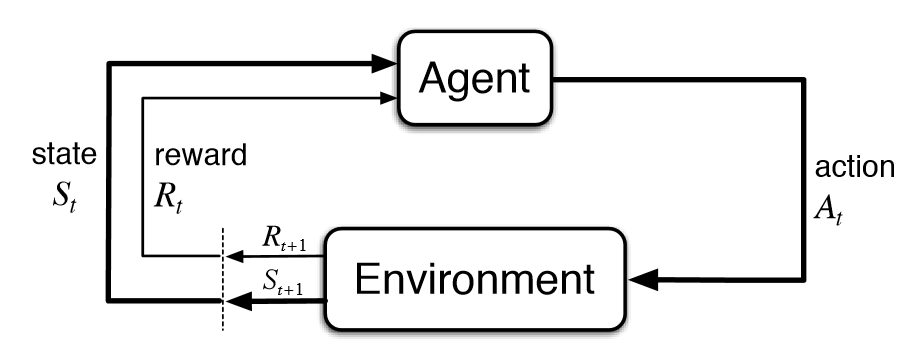
\includegraphics[width=0.8\textwidth]{./figures/rl.png}
    \caption{ Reinforcement Learning Illustration}
    \label{fig:RL}
\end{figure}


Figure \ref{fig:RL} shows the basic model of reinforcement learning. At each time $t$, an agent
receives the environment state $S_t$ and current reward $R_t$. It then chooses an action $a_t$
from the set of available actions, which is sent to the environment. The environment moves
to a new state $S_{t+1}$ and new reward $R_{t+1}$ and feedback to the agent. The goal of a
reinforcement learning agent is to gain as much as reward as possible.


In this proposed project, we will use the method of deep Q-learning. Q-learning defines a reward
expectation function, $Q$, which provides the expected reward of an action $a$ taken under the
current state $s$. This $Q$ function can be recursively defined as $Q(s,a) = R(s,a) + \alpha
\max_{a^{'}} Q(S^{'}(s,a),a^{'})$, where $R$ is the immediate reward given action $a$ taken under
state $s$, $\alpha$ is the discount rate of future reward and $S^{'}$ is the state transition.
Given numerous possibilities of imagery state $s$, we cannot compute $Q$ directly. Alternatively,
we can use a deep convolutional network to estimate $Q$.

TODO CNN description\\

\section{Design of experiments and performance evaluation}

We run several random episodes of the Enduro game simulator and store all the observations and rewards.

TODO Performance evaluation\\
TODO Comparison with other model\\

\section {Project planning}

\begin{center}
    \begin{tabular}{ | c | c | c | } 
        \hline
        Timeline & Project Task & Work Distribution   \\ 
        \hline
        Oct 25   & system setup &   \\ 
        \hline
        Oct 30   & data generation and proprocessing &   \\ 
        \hline
        Nov 15   & algorithm  &   \\ 
        \hline
        Nov 25   & evaluation  &   \\ 
        \hline
        Nov 30   & report and video  &   \\ 
        \hline
    \end{tabular}
\end{center}


TODO References\\
% \begin{figure}
% \centering
% \includegraphics[width=0.3\textwidth]{frog.jpg}
% \caption{\label{fig:frog}This frog was uploaded to writeLaTeX via the project menu.}
% \end{figure}


\begin{thebibliography}{9}
\bibitem{google}
  Google Self-Driving Car, \texttt{https://www.google.com/selfdrivingcar}

\bibitem{tesla}
  Tesla Self-Driving Hardware, \texttt{https://www.tesla.com/autopilot}

\bibitem{gym}
  OpenAI Gym toolkit, \texttt{https://gym.openai.com}

\bibitem{enduro}
  OpenAI Gym Enduro Environment, \texttt{https://gym.openai.com/envs/Enduro-v0}

\end{thebibliography}
\end{document}
